\documentclass[a4paper,12pt]{report} % Tipo di documento
\usepackage[utf8]{inputenc}           % Codifica
\usepackage[T1]{fontenc}              % Font moderni
\usepackage[italian]{babel}
\usepackage{amsmath,amssymb,amsfonts} % Pacchetti per matematica
%\usepackage{siunitx}                  % Unità di misura
\usepackage{physics}                  % Simboli fisici
\usepackage{graphicx}                 % Inserire immagini
\usepackage{pgfplots}
\pgfplotsset{compat=1.18}
\usepackage{float}                    % Gestione di immagini/flottanti
\usepackage{xcolor}                   % Colori personalizzati
\usepackage{hyperref}                 % Link cliccabili
\usepackage{geometry}                 % Personalizzazione margini
\geometry{margin=2.5cm}               % Margini di 2.5 cm
\usepackage{tikz}                     % Disegni e diagrammi
\usepackage[version=4]{mhchem}                   % Chimica, per formule come \ce{H2O}
\usepackage{booktabs}                 % Tabelle migliorate
\usepackage{cancel}                   % Per cancellare termini (\cancel{})
\usepackage{enumitem}                 % Liste personalizzate
%\usepackage{multicol}                 % Layout a colonne
\usepackage{fancyhdr}                 % Intestazioni e piè di pagina
\setlength{\headheight}{14.5pt}
\pagestyle{fancy}                     % Abilita intestazioni/piè di pagina
\fancyhead[L]{Appunti di Analisi I}      % Testo a sinistra nell'intestazione
\fancyhead[R]{\today}                 % Data a destra
\fancyfoot[C]{\thepage}               % Numerazione delle pagine al centro
\renewcommand{\baselinestretch}{1.2}  % Interlinea
\usepackage{xcolor}
\DeclareEmphSequence{\bfseries\itshape}
\newcommand{\mean}[1]{\langle #1 \rangle}

\title{Appunti di Analisi I}
\author{Alessandro Consoli, Sonia Facciolà e Joey Butchers}
\date{Anno 2024/2025}

\begin{document}

    \begin{titlepage}
    \begin{center}
        \begin{minipage}[ht!]{0.49\textwidth}
                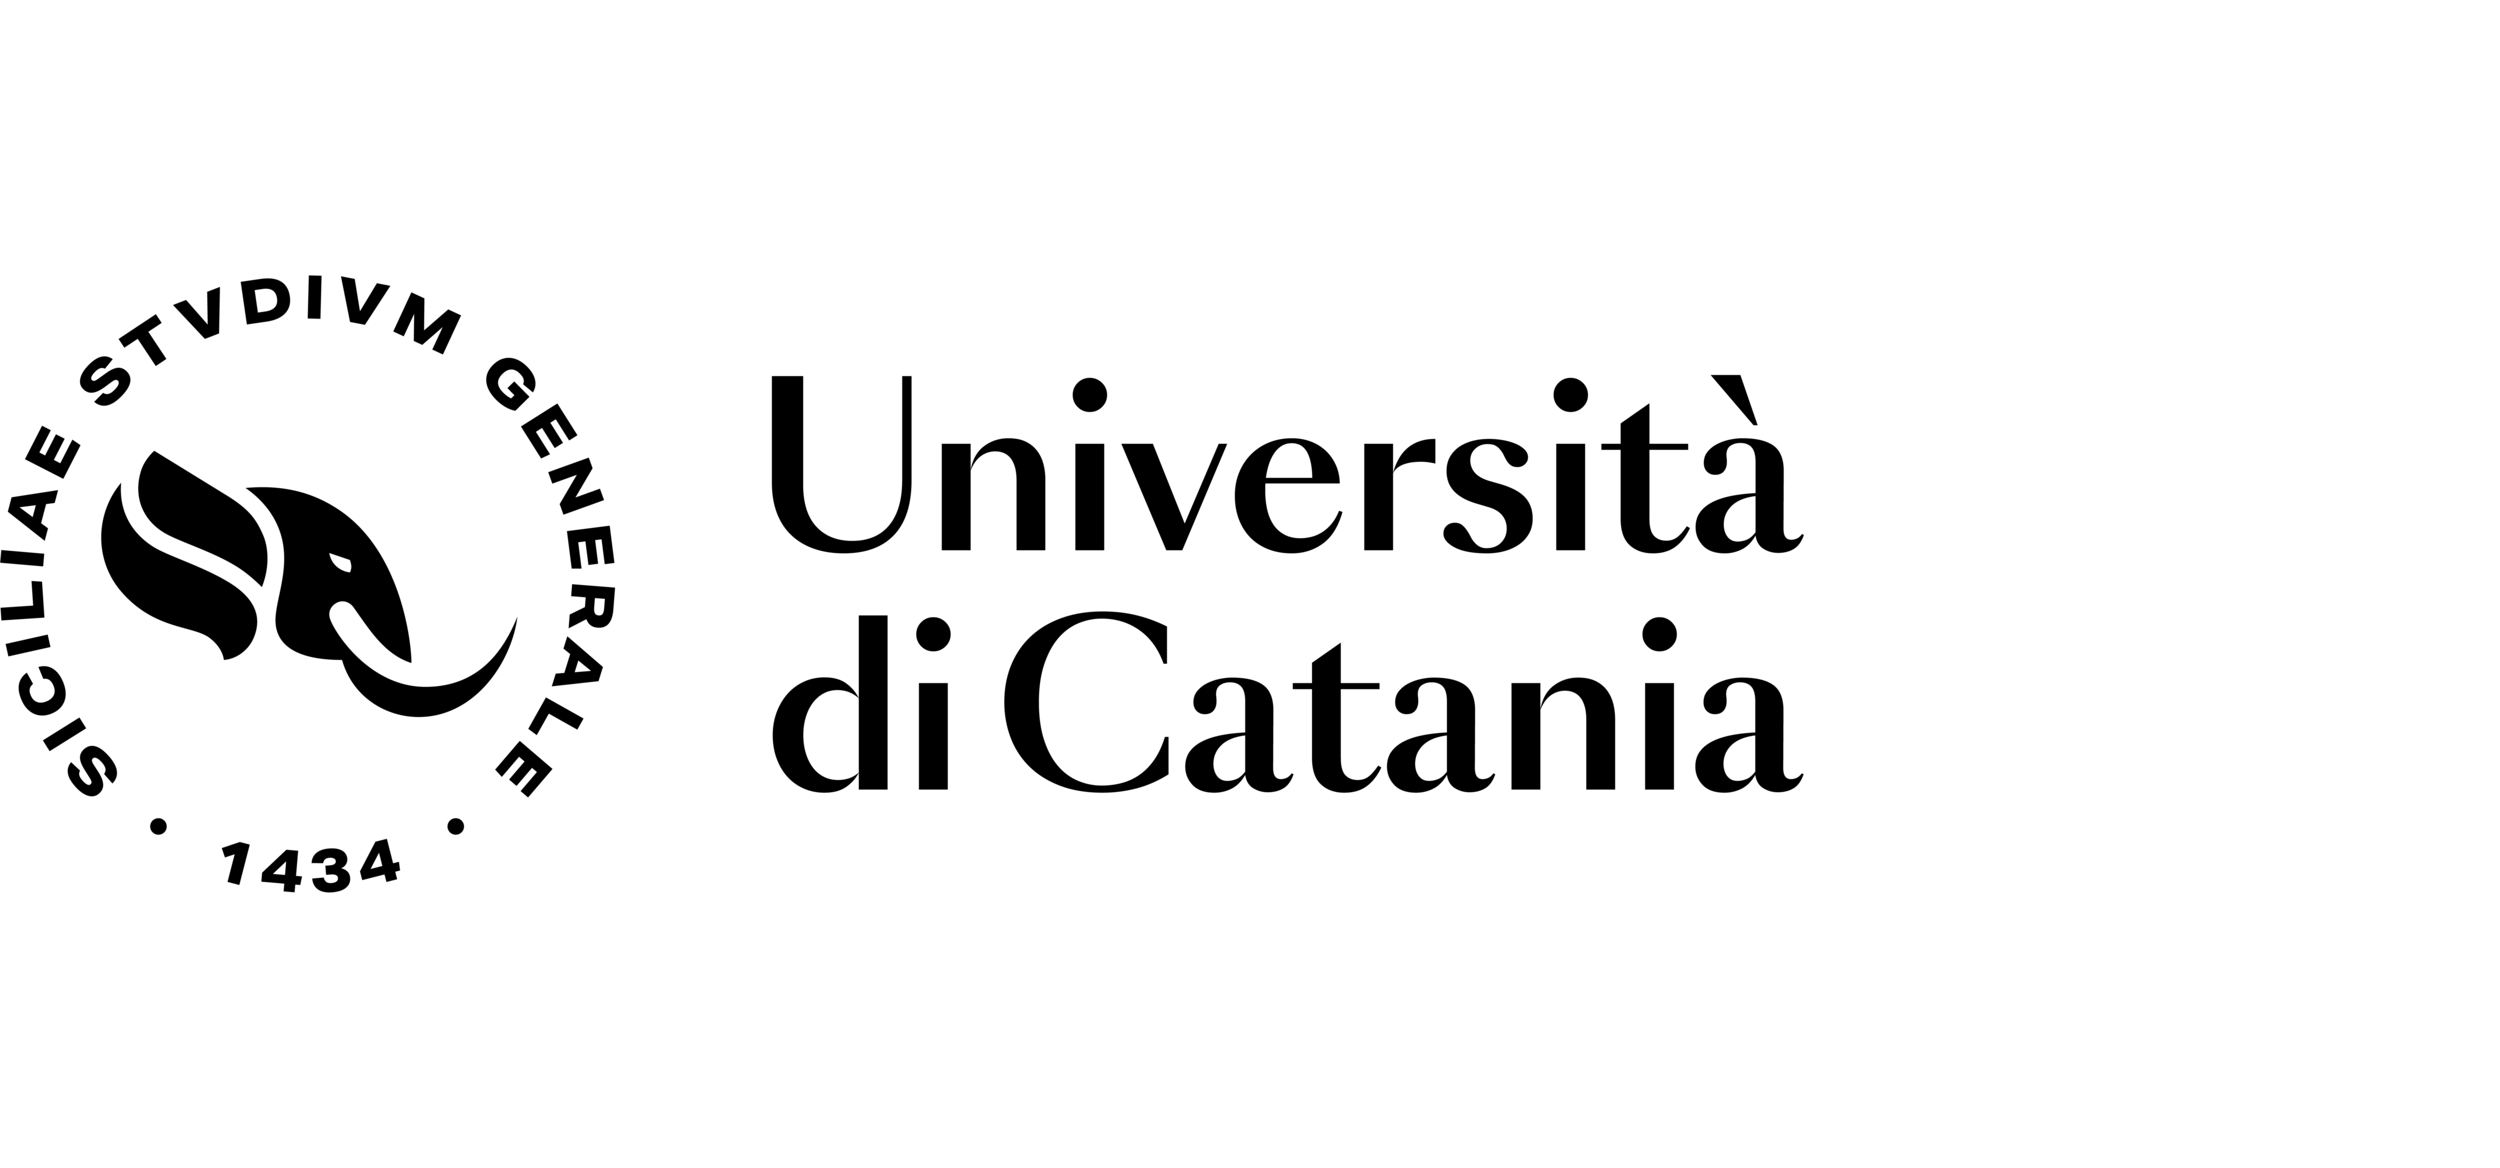
\includegraphics[width=\textwidth]{images/Logo+UniCT.png}
        \end{minipage}
        \hfill
        \begin{minipage}[th!]{0.49\textwidth}
                
\includegraphics[width=\textwidth]{images/LogoDfa2.png}
        \end{minipage}
        \large
        \textbf{CORSO DI LAUREA IN FISICA}
        \vspace{0.5cm}
        \hrule
        \vspace{3cm}
        \centering
        \textbf{Alessandro Consoli\\Sonia Facciolà\\Joey Butchers}\\
        \vspace{1cm}
        \Huge{\textbf{Appunti di Analisi I}}\\
        
        \vfill
        
        \begin{minipage}[h]{0.35\textwidth}
            \hrule
            \vspace{0.3cm}
            \small \centering
            Appunti di Analisi I
            \vspace{0.35cm}
            \hrule
        \end{minipage}
        
        \vfill
        
        \hrule
        \vspace{0.3cm}
        \normalsize
        \textbf{Anno Accademico 2024/2025}
    \end{center}

    
\end{titlepage}
    
    \tableofcontents


    \maketitle
    
\chapter{Funzioni e Insiemi numerici}

    \section{introduzione}

        Presi due insiemi $X$ e $Y$ e $f$ una funzione che associa ad ogni elemento 
    di $X$ \emph{uno e uno solo} elemento di $Y$, la terna ordinata $(X,Y,f)$ è detta funzione.
    Il primo insieme è detto \emph{dominio} della funzione, il secondo \emph{codominio} e 
    l'insieme dei valori che la funzione assume è detto \emph{immagine} della funzione. Per indicare la funzione si usa la notazione:
        \begin{equation}
            f: X \to Y
        \end{equation}
        dove $x$ indica il generico elemento di $X$ e $f(x)$ il corrispondente elemento di $Y$.
        Se $f(x_0)=y_0$ si dice che $y_0$ è l'immagine di $x_0$ e si scrive $y_0=f(x_0)$. 
        \\\\ \emph{Definizione di prolungamento}: 
        \begin{definizione} di una funzione: siano $X,Y,Z$ tre insiemi e $f: X \to Y$ e $g: Y \to Z$ due funzioni. Si dice che $g$ è il prolungamento di $f$ se:
        \begin{equation}
            g(x)=g(f(x)) \quad \forall x \in X
        \end{equation}
    \end{definizione}
    \vspace{0.1cm} % Adjust the spacing to avoid the empty box issue
    \emph{Definizione di funzione suriettiva}: 
    \begin{definizione} 
        si dice suriettiva se ogni elemento del codominio $Y$ ha almeno un elemento nel dominio $X$ che lo mappa su di esso:
        \begin{equation}
            \forall y \in Y \quad \exists x \in X \quad \text{tale che} \quad f(x)=y
        \end{equation}  
    \end{definizione}
    \emph{Definizione di funzione iniettiva}: 
    \begin{definizione} si dice iniettiva se ad ogni elemento del dominio $X$ corrisponde un solo elemento del codominio $Y$:
        \begin{equation}
            \forall x_1,x_2 \in X \quad \text{tali che} \quad x_1 \neq x_2 \quad \text{allora} \quad f(x_1) \neq f(x_2)
        \end{equation}
    \end{definizione}
\begin{definizione}
    Diciamo che $f$ ha una corrispondenza biunivoca tra $X$ e $Y$ se è sia suriettiva che iniettiva.
\end{definizione}

\begin{esempio}
    \begin{itemize}
        \item $f(x)=x^2$ è una funzione suriettiva ma non iniettiva.
        \item $f(x)=x^3$ è una funzione suriettiva e iniettiva.
        \item $f(x)=\sin(x)$ è una funzione suriettiva ma non iniettiva.
        \item $f(x)=\exp(x)$ è una funzione suriettiva e iniettiva(corrispondeza biunivoca).
    \end{itemize}
\end{esempio}
\section{Relazioni di equivalenza}
         \label{sec:Relazioni_di_equivalenza} 

             Una relazione di equivalenza è una relazione binaria $\sim$ su un insieme $X$ che soddisfa le seguenti proprietà:
        \begin{definizione}
             \begin{itemize}
                  \item \emph{Riflessiva}: $\forall x \in X, \; x \, \sim \, x$
                   \item \emph{Simmetrica}: $\forall x, y \in X, \; x \, \sim \, y \implies y \, \sim \, x$
                  \item \emph{Transitiva}: $\forall x, y, z \in X, \; x \, \sim \, y \land y \, \sim \, z \implies x \, \sim \, z$
              \end{itemize}
        \end{definizione}
        \emph{Definizione di classe di equivalenza}:
    \begin{definizione} 
          sia $\sim$ una relazione di equivalenza su un insieme $X$ e $x \in X$. La classe di equivalenza di $x$ rispetto a $\sim$ è l'insieme:
            \begin{equation}
                 [x] = \{y \in X \; | \; y \, \sim \, x\}   
             \end{equation}
    \end{definizione}
        \emph{Definizione di insieme quoziente}:
    \begin{definizione}
                sia $\sim$ una relazione di equivalenza su un insieme $X$. L'insieme quoziente di $X$ rispetto a $\sim$ è l'insieme:
                \begin{equation}
                    X/\sim = \{[x] \; | \; x \in X\}
                \end{equation}
     \end{definizione} 
         \emph{Definizione di funzione di proiezione}:
    \begin{definizione} 
            sia $\sim$ una relazione di equivalenza su un insieme $X$. La funzione di proiezione è la funzione:
            \begin{equation}
                 \pi: X \to X/\sim \quad \text{tale che} \quad \pi(x) = [x]
          \end{equation}
    \end{definizione}
    \emph{Definizione di funzione inversa}:
    \begin{definizione} 
        sia $f: X \to Y$ una funzione. Si dice che $f$ è invertibile se è suriettiva e iniettiva. In tal caso diciamo che è invertibile e che la sua inversa è $f^{-1}: Y \to X$ tale che:
        \begin{equation}
            y=f^{-1}(x) \quad \forall x \in X
        \end{equation}
    \end{definizione}
\subsection{Funzioni Monotòne}
Parlando di monotonia di una funzione nel suo insieme $A$ possiamo distinguere 4 casi:
    \begin{definizione}
        Diciamo che una funzione $f: A \to \mathbb{R}$ è monotòna se $\forall{x_1, x_2}$ $\in A$ vale:
    \end{definizione}
\begin{align}
    &f \text{ è crescente in } A \text{ se } x_1 < x_2 \implies f(x_1) \leq f(x_2) \\
    &f \text{ è strettamente crescente in } A \text{ se } x_1 < x_2 \implies f(x_1) < f(x_2) \\
    &f \text{ è decrescente in } A \text{ se } x_1 < x_2 \implies f(x_1) \geq f(x_2) \\
    &f \text{ è strettamente decrescente in } A \text{ se } x_1 < x_2 \implies f(x_1) > f(x_2) \\
    &f \text{ è costante in } A \text{ se } x_1, x_2 \in A \implies f(x_1) = f(x_2)
\end{align}
\begin{esempio}
    \begin{itemize}
        \item $f(x)=x^2$ è strettamente crescente in $\mathbb{R}^+$
        \item $f(x)=x^3$ è crescente in $\mathbb{R}$
        \item $f(x)=\sin(x)$ è crescente in $\left[-\frac{\pi}{2},\frac{\pi}{2}\right]$
        \item $f(x)= e^{x}$ è strettamente crescente in $\mathbb{R}$
    \end{itemize}
\end{esempio}

\chapter{Campo Complesso}

    \section{Campo Complesso}

    Visto che \emph{$\mathbb{R}$ non è algebricamente chiuso}(vale a dire che non tutti i polinomi hanno radici in $\mathbb{R}$).\`E possibile estendere il campo dei numeri reali in modo da includere le radici di tutti i polinomi. Questo campo è il campo dei numeri complessi, indicato con $\mathbb{C}$.
\section{Definizione}
Per definire un campo, vanno a loro volta definite 2 oparazioni e soddisfatte 9 proprioetà.\\
\begin{itemize}
    \item $(a,b) + (c,d) = (a+c,b+d)$ $\to$ operazione di $\mathbb{R}$ già nota.
    \item $(a,b) * (c,d) = (ac-bd,ad+bc)$
    \item elemento neutro $0$ = (1,0)
    \item inverso? $\to$ prendiamo $(a,b) \neq (0,0) \to \exists (x,y) : (a,b)(x,y)=(1,0) \to (ax-by,ay+bx)=(1,0) \to ax-by=1 \land ay+bx=0 \to x=\frac{a}{a^2+b^2} \land y=\frac{-b}{a^2+b^2}$
\end{itemize}


\chapter{Limiti di Funzioni}

    \section{Limiti di Funzioni}

    \input{chapters/limiti_di_funzioni/limiti_di_funzioni.tex}



\chapter{Funzioni Continue}

    \section{Funzioni Continue}
    
    


Per definire una funzione continua e parlare quindi continuità di una funzione dobbiamo
definire delle condizioni che la funzione dovrà rispettare per essere definita continua in un punto: partendo da questo preambolo:
    \begin{equation}
        f(x):X \to Y \quad x_0 \in X
    \end{equation}
le condizioni sono:
    \begin{equation}
        \text{1)} \exists f(x_0) \qquad \text{2)} \exists \lim_{x \to x_0} f(x)=l \in \mathbb{R} \qquad \text{3)} f(x_0)=l
    \end{equation}
    
    

\chapter{limiti notevoli, derivate notevoli, sviluppi di Taylor notevoli}

limiti notevoli
\section{Limiti Notevoli}   
$\lim\limits_{x \to 0} \frac{\sin x}{x} = 1$ \qquad \qquad \qquad \qquad
$\lim\limits_{x \to 0} \frac{1 - \cos x}{x} = 0$ \qquad \qquad \qquad \qquad
$\lim\limits_{x \to 0} \frac{e^x - 1}{x} = 1$\\
$\lim\limits_{x \to 0} \frac{\log(1 + x)}{x} = 1$ \qquad \qquad \qquad \qquad
$\lim\limits_{x \to 0} \frac{a^x - 1}{x} = \log a$ \qquad \qquad \qquad \qquad
$\lim\limits_{x \to 0} \frac{x}{\tan x} = 1$\\
$\lim\limits_{x \to 0} \frac{\tan x}{x} = 1$ \qquad \qquad \qquad \qquad
$\lim\limits_{x \to 0} \frac{\operatorname{arctanh} x}{x} = 1$ \qquad \qquad \qquad \qquad
$\lim\limits_{x \to 0} \frac{\arctan x}{x} = 1$\\
$\lim\limits_{x \to 0} \frac{\log(1 + x)}{x^2} = \frac{1}{2}$ \qquad \qquad \qquad \qquad
$\lim\limits_{x \to 0} \frac{\log(1 + x)}{x} = 1$ \qquad \qquad \qquad \qquad
$\lim\limits_{x \to 0} \frac{1 - \cos x}{x^2} = \frac{1}{2}$\\
$\lim\limits_{x \to 0} \frac{e^x - 1}{x^2} = 1$ \qquad \qquad \qquad \qquad
$\lim\limits_{x \to 0} \frac{\log(1 + x)}{x^2} = \frac{1}{2}$ \qquad \qquad \qquad \qquad
$\lim\limits_{x \to 0} \frac{a^x - 1}{x^2} = \log a$\\
$\lim\limits_{x \to 0} \frac{\sin x}{x^2} = \frac{1}{6}$ \qquad \qquad \qquad \qquad
$\lim\limits_{x \to 0} \frac{\tan x}{x^2} = \frac{1}{3}$ \qquad \qquad \qquad \qquad
$\lim\limits_{x \to 0} \frac{\arcsin x}{x^2} = \frac{1}{6}$\\
$\lim\limits_{x \to 0} \frac{\arctan x}{x^2} = \frac{1}{3}$ \qquad \qquad \qquad \qquad




    \end{document}
    